%%*****************************************************************************
\SVN$Id$
%%*****************************************************************************
%%
%% Copyright (C) 2005-2009 The ExTeX Group and individual authors listed below
%%
%% This library is free software; you can redistribute it and/or modify it
%% under the terms of the GNU Lesser General Public License as published by the
%% Free Software Foundation; either version 2.1 of the License, or (at your
%% option) any later version.
%%
%% This library is distributed in the hope that it will be useful, but WITHOUT
%% ANY WARRANTY; without even the implied warranty of MERCHANTABILITY or
%% FITNESS FOR A PARTICULAR PURPOSE. See the GNU Lesser General Public License
%% for more details.
%%
%% You should have received a copy of the GNU Lesser General Public License
%% along with this library; if not, write to the Free Software Foundation,
%% Inc., 59 Temple Place, Suite 330, Boston, MA 02111-1307 USA
%%
%%*****************************************************************************
%% @author Gerd Neugebauer
%%-----------------------------------------------------------------------------
\chapter{Source Code Documentation}


The source code has to be documented. \TeX\ shows us a good example of
a proper documenatation. Donald Knuth\index{Knuth!Donald} has invented
the Web system to keep together the documentation and the source code.
This is called \+literate programming+. The source code and
documentation are extracted from a common file. In the Java world the
\+Javadoc+ system has been invented for a similar purpose.


\section{Javadoc}\index{Javadoc|(}

The Javadoc conventions for comments make it possible to extract the
relevant part of the documentation and generate several outut formats
from it. The primary output format is HTML.
\begin{figure}[tbh]
  \centering
  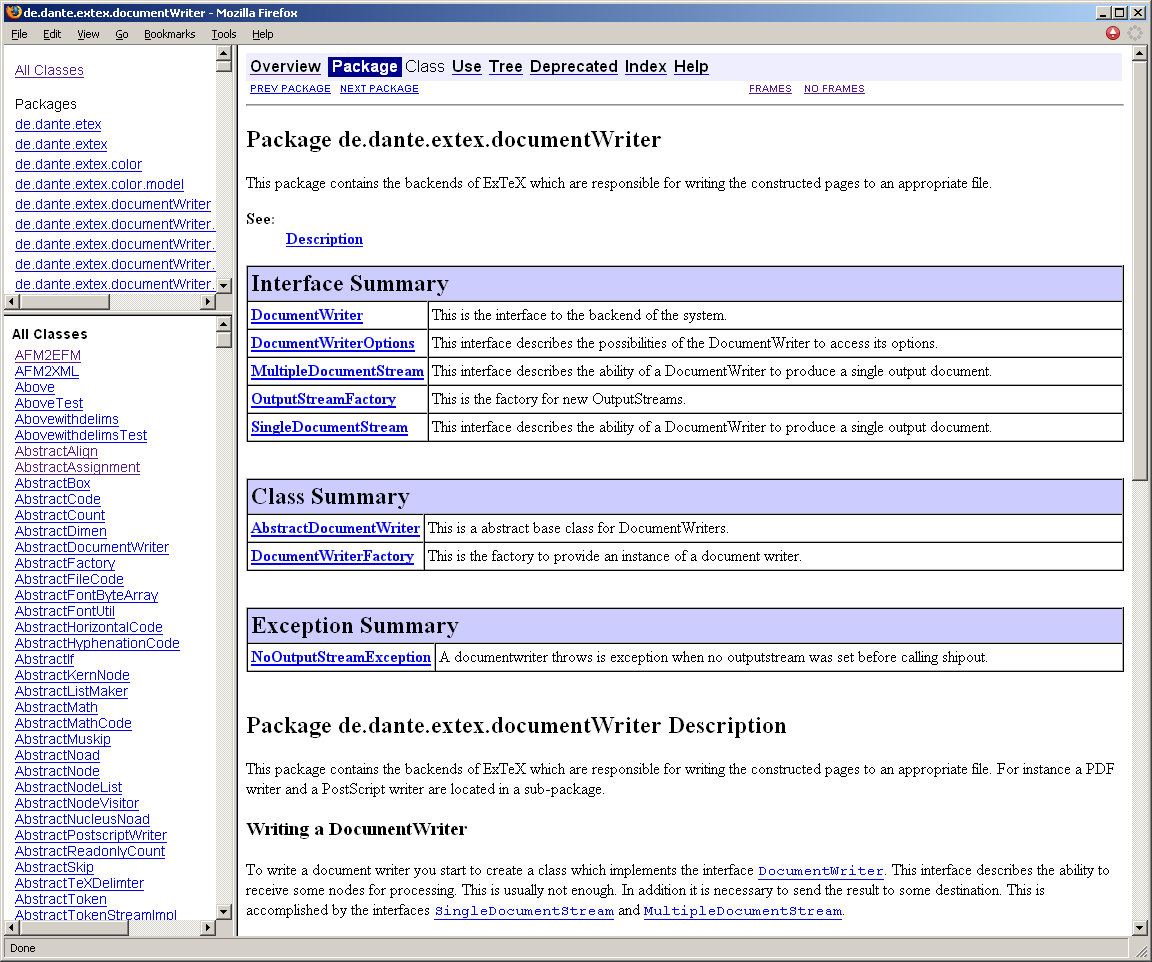
\includegraphics[scale=.33]{image/javadoc}
  \caption{Javadoc in the Browser}\label{fig:eclipse-javadoc}
\end{figure}
\index{Javadoc|)}


\section{Documentation of Primitives}

The documentation of the primitives is contained in the \+Javadoc+
comments of the implementing Java classes. A script is used to extract
the information from the sources for the \textit{User's Manual}. To
make this happen, the documentation meant for the manual has to be
marked and formatted specially.

\INCOMPLETE


